\subsection{Pagina de registo}

Esta página permite que os utilizadores não registados, efetuem o registo no sistema para poderem aceder a todas as funcionalidades.\\

Para efetuar o registo, um utilizador apenas precisa de indicar os campos essenciais para utilizar o sistema, nome, email, número de aluno (se indicar que é estudante), telemóvel e \textit{password}.
Os restantes campos que compõem a informação do utilizador, como descrição e fotografia, podem ser preenchidos posteriormente, na edição do perfil.\\

Depois do registo, os utilizadores serão direcionados para o painel do aluno ou docente, dependendo do tipo de utilizador que indicou.

Nesta página os utilizadores não autenticados podem regressar à página inicial, ao carregar no logótipo do sistema, ou aceder à página de autenticação.

O utilizador é notificado com mensagens de erro explicitas quando falhar o registo, indicando em que campo(s) ocorreram erros. 

Para esta página procurou-se um \textit{design} simples, onde o utilizador pode concentrar-se exclusivamente na funcionalidade pretendida, o registo.\\

Na Figura~\ref{fig:sign_up} pode ser consultada uma imagem demonstrativa da página desenvolvida.\\

\begin{figure}[H]
  \centering
  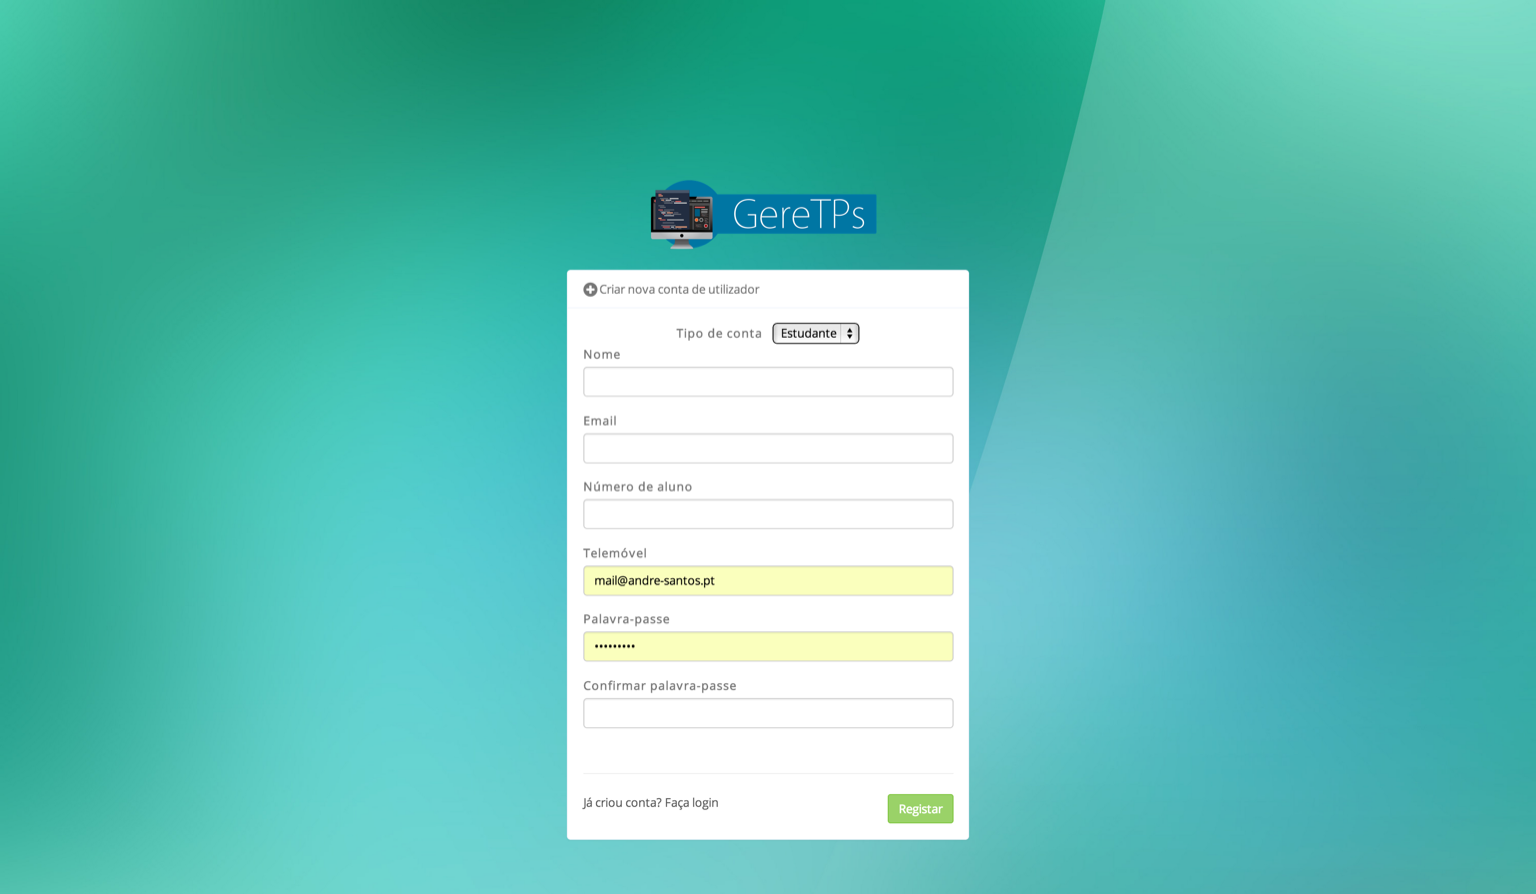
\includegraphics[width=1\textwidth,center]{images/implementacao/sign_up}
  \caption{Página de registo}
  \label{fig:sign_up}
\end{figure}
